\subsection{Algoritmo}
Para resolver el problema de forma exacta, se utiliza la técnica algorítmica \textit{Backtracking}, la cual consiste en realizar una búsqueda exhaustiva entre todas las posibles soluciones al problema.

En nuestro caso, esta técnica genera todas las cliques posibles y para cada una de ellas se calcula su frontera. Por cada nueva frontera calculada, se compara con el mejor resultado ya obtenido, y de hallar uno mejor, lo reemplaza.

Esto se realiza de forma recursiva, a través de la función MaximaFrontera, la cual toma una lista de nodos que es potencialmente una clique, y un nodo. Esta función se llama inicialmente con una lista de nodos vacía y con el primer nodo. Para cada llamado, la función analiza la lista recibida. En caso de ser clique, calcula su frontera y la compara con los valores máximos ya obtenidos, actualizando estos últimos en caso de encontrar una mejor solución. Luego, se llama recursivamente avanzando al siguiente nodo tomando las dos opciones posibles: agregarlo o no agregarlo. De esta forma, se van generando todos los conjuntos de nodos posibles y se lo estudia a cada uno.

De todas formas, si se determina que una lista de nodos no es clique, se descarta la rama (a menos que sea una lista vacía), ya que agregar nuevos nodos no puede recuperar la propiedad de ser clique. Esto hace que no se recorran todos los conjuntos posibles de nodos, sino los que son potencialmente cliques.

Esto finaliza cuando ya se recorrieron todos los nodos y por lo tantos se formaron todas las cliques posibles.

El algoritmo mencionado se puede ver en el siguiente pseudocódigo:

\begin{algorithm}[H]
\begin{algorithmic}
\caption{Algoritmo exacto.}
	\Function{MaximaFrontera}{clique, nodo} \\
		\State{}
		\eIf {seAgregoUnNodo $\wedge$ esClique(clique)}{
			tamFrontera $\leftarrow$ TamañoFrontera(clique)\;
			
			\If {tamFrontera > maxFrontera}{
				ActualizarMaximos(clique, tamFrontera)
			}
		}{
			\If {seAgregoUnNodo}{
			retornar			
			}
		}
		
		\State{}
		\If {recorrí todo los nodos}{
			retornar		
		}
		
		\State{}
		maximaFrontera(clique, nodo+1) \;
		clique.Agregar(nodo) \;
		maximaFrontera(clique, nodo+1) \;
	\EndFunction
\end{algorithmic}
\end{algorithm}

Algo importante de destacar sobre este algoritmo es que en toda llamada la lista de nodos que se recibe es una potencial clique. Esto se debe a que, por como fue construida, todos los nodos de la lista, excepto el último, forman una clique. De no serlo, en el llamado anterior, al determinar que no era clique, no se hubiese continuado y agregado un nodo a esa lista.

Por este motivo, determinar si una lista de nodos (o potencial clique) es una clique consiste únicamente en ver si el último nodo es adyacente a todos los anteriores, lo cual reduce considerablemente la complejidad de la función.

Para evitar controlar innecesariamente si una lista de nodos es clique luego de no haber agregado nada en la iteración anterior (y por lo tanto es necesariamente clique porque en la iteración anterior lo era), el algoritmo verifica en un comienzo si algo fue agregado, y solo en caso afirmativo chequea si se trata de una clique. En caso contrario, saltea el paso asumiendo que ya lo realizó en la iteración anterior.

Este paso mencionado se realiza sencillamente verificando que el último nodo de la lista es el anterior al nodo actual (nodo-1), ya que la lista va a haber cambiado de la iteración anterior si es que se agregó ese nodo.


\subsection{Complejidad}

Al tratarse de una función recursiva, la complejidad se divide en dos partes: los llamados recursivos y el costo de cada llamado.

En cuanto a la primera parte, en cada llamado hay 2 opciones posibles:

\begin{itemize}
\item La potencial clique no resulta ser clique y se descarta la rama.
\item La potencial clique resulta ser clique, y se avanza al siguiente nodo sin agregar el nodo actual en una rama, y agregándolo en otra.
\end{itemize}

En el peor caso, es decir cuando la lista de nodos resulta ser clique, se realizan dos llamados recursivos y así se van generando todos los conjuntos de potenciales cliques. La cantidad de estos subconjuntos es $2^n$ donde $n$ es la cantidad de nodos, ya que cada nodo tiene dos opciones: estar o no estar. Por lo tanto, el costo de los llamados recursivos es $O(2^n)$.

Notar que este peor caso puede suceder, ya que en un grafo completo (y por lo tanto clique), todo subconjunto de nodos es también clique.

El peor caso en un llamado recursivo se presenta cuando la potencial clique recibida es efectivamente clique (y se ha agregado un nodo en la iteración anterior, ya que en caso contrario, no hace falta estudiar ese caso). Esto se debe a que no solo hay que determinar si es clique, sino que, además, luego hay que calcular el tamaño de la frontera para poder compararlo con el máximo ya obtenido. Por lo tanto, el costo en peor caso en un llamado es precisamente el costo de determinar si es una lista es clique más el costo de calcular su frontera.

Como se mencionó previamente, como la lista de nodos recibida es una potencial clique, para determinar si es efectivamente una clique solo hay que verificar que el último nodo sea adyacente a los anteriores. Esto tiene un costo $O(k)$, siendo $k$ el tamaño de la lista, o simplemente $O(n)$, ya que con matriz de adyacencias determinar si dos nodos son adyacentes es $O(1)$.

En cuanto a calcular el tamaño de la frontera, hay que sumar la cantidad de adyacencias de cada nodo de la clique, es decir, para cada nodo de la clique ($O(k)$) se compara contra todo nodo ($O(n)$) para ver si es adyacente ($O(1)$) y de ser así se agrega al contador. Finalmente se restan la cantidad de adyacencias que son internas a la clique ($k*(k-1)$, cada nodo de la clique se conecta con todos menos sí mismo). Por lo tanto, el costo de este paso es $O(k*n*1)$ o simplemente $O(n^2)$.

Finalmente, el costo de cada llamado recursivo es $O(n)$ + $O(n^2)$ = $O(n^2)$.

Habiendo calculado tanto el costo de realizar los llamados recursivos como el costo de cada uno de ellos, solo resta multiplicar ambos costos. Así, el costo total en peor caso del algoritmo es $O(2^n)$*$O(n^2)$ = $O(2^n.n^2)$.

\subsection{Experimentación}

La experimentación sobre el algoritmo exacto consiste en medir los tiempos\footnote{Para las mediciones de tiempo se utilizó la librería chronos de C++.} de cómputo para grafos de distintos tamaños. Todas las mediciones fueron realizadas 5 veces y luego los resultados promediados.

Estos grafos fueron generados de forma pseudo-aleatoria\footnote{ Para todas las decisiones aleatorias se utilizó la función rand() de C++.} con una herramienta que toma dos valores como parametro: $n$ \textit{($>$ 10)} y $d$ \textit{(entre 0 y 10)}. Esta crea un grafo de $n$ nodos y toma $n*d/10$ de esos nodos y los conecta entre si formando cliques disjuntas de tamaño aleatorio. Luego conecta nodos al azar de forma que cada posible arista tiene una probabilidad de $d/10$ de estar en el grafo. De esta forma con $d=0$ se generaría un grafo con $n$ nodos aislados, y con $d=10$ un grafo completo.

El objetivo de este experimento es comprobar de forma empirica como se comporta el algoritmo en función del tamaño de entrada. Además se espera que otorgue información útil para los experimentos subsiguientes cuando querramos comparar los resultados obtenidos con otros métodos con el resultado exacto, y así saber con grafos de que tamaño experimentar en función del tiempo que estemos dispuestos a dedicar.

\begin{figure}[h]
	\centering
		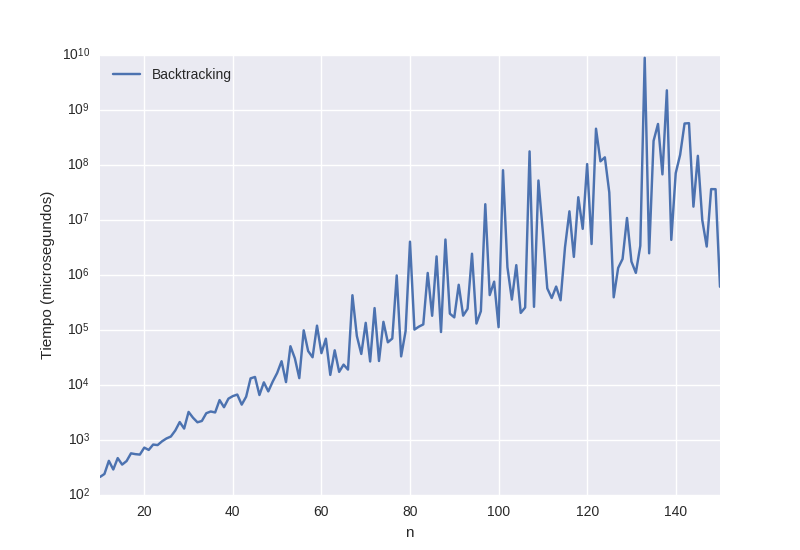
\includegraphics[scale=0.6]{Imagenes/Tiempos150nlogy.png}
		\caption{\small{Tiempos de cómputo del algoritmo exacto según cantidad de nodos.}}
        \label{backtrackingN}
\end{figure}

En la figura \ref{backtrackingN} se puede observar el resultado de las mediciones. Tal como era esperable, los tiempos de cómputo aumentan de forma exponencial según el tamaño de entrada. Sin embargo, presenta variaciones significativas dadas por alguna otra variable. 

Observando algunos de los grafos que llevaron mayor tiempo resolver, notamos que tenían mayor cantidad de aristas ($m$) que sus vecinos en $n$, por lo que analizamos la posibilidad de que la cantidad de aristas afecte de forma más directa a la complejidad del algoritmo que la cantidad de nodos. Esto es posible ya que por como fueron generados los grafos, la relación entre cantidad de nodos y aristas es solo directa en probabilidad, y presenta variaciones aleatorias. En la figura \ref{backtrackingM} se grafican los mismos datos, pero ordenados según cantidad de aristas, y se puede observar que presentan aún más variación que la figura anterior. 

Por lo tanto las variables que afectan a la complejidad del algoritmo, además de $n$ y $m$, deben deberse a alguna otra caractéristica de los grafos más difícil de caracterizar, como puede ser por ejemplo la cantidad total de cliques.

\begin{figure}[h!]
	\centering
		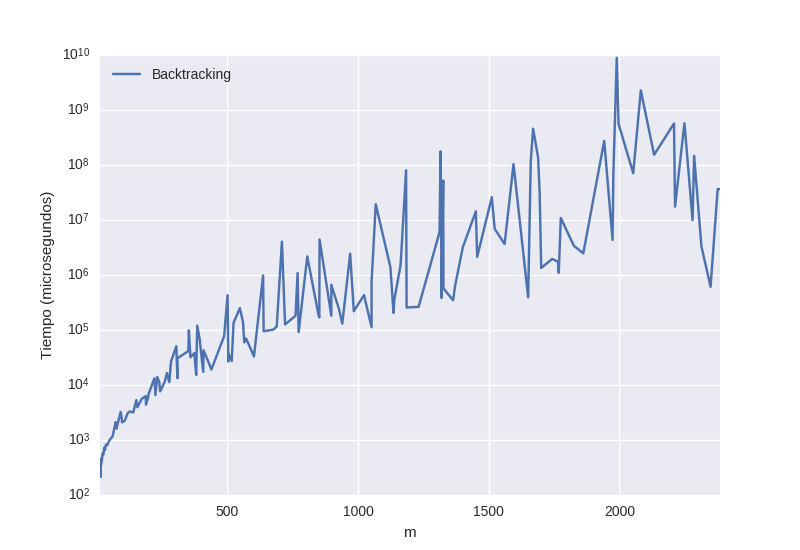
\includegraphics[scale=0.6]{Imagenes/Tiempos150mlogy.png}
		\caption{\small{Tiempos de cómputo del algoritmo exacto según cantidad de aristas.}}
        \label{backtrackingM}
\end{figure}